% The Clever Algorithms Project: http://www.CleverAlgorithms.com
% (c) Copyright 2010 Jason Brownlee. Some Rights Reserved. 
% This work is licensed under a Creative Commons Attribution-Noncommercial-Share Alike 2.5 Australia License.

% This is a chapter

\renewcommand{\bibsection}{\subsection{\bibname}}
\begin{bibunit}

\chapter{Regression}
\label{ch:regression}
\index{Regression}

\section{Overview}
This chapter describes Regression.


% Strategy: Problem solving plan
% The strategy is an abstract description of the computational model. The strategy describes the information processing actions a technique shall take in order to achieve an objective. The strategy provides a logical separation between a computational realization (procedure) and a analogous system (metaphor). A given problem solving strategy may be realized as one of a number specific algorithms or problem solving systems. The strategy description is textual using information processing and algorithmic terminology.
\subsection{Strategy}
% What is the information processing objective of a technique?
% What is a techniques plan of action?

stats?

here we take a machine learning / data mining perspective. 

earth r package?

types:
Linear Regression
Non-Linear Regression
Generalized Linear Regression

% Heuristics: Usage guidelines
% The heuristics element describe the commonsense, best practice, and demonstrated rules for applying and configuring a parameterized algorithm. The heuristics relate to the technical details of the techniques procedure and data structures for general classes of application (neither specific implementations not specific problem instances). The heuristics are described textually, such as a series of guidelines in a bullet-point structure.
\subsection{Heuristics}
% What are the suggested configurations for a technique?
% What are the guidelines for the application of a technique to a problem instance?

\begin{itemize}
	\item 
\end{itemize}



% References: Deeper understanding
% The references element description includes a listing of both primary sources of information about the technique as well as useful introductory sources for novices to gain a deeper understanding of the theory and application of the technique. The description consists of hand-selected reference material including books, peer reviewed conference papers, journal articles, and potentially websites. A bullet-pointed structure is suggested.
\subsection{References}
% What are the primary sources for a technique?
% What are the suggested reference sources for learning more about a technique?

% primary sources
\subsubsection{Primary Sources}


% more info
\subsubsection{More Information}




\putbib
\end{bibunit}

\newpage\begin{bibunit}% The Clever Algorithms Project: http://www.CleverAlgorithms.com
% (c) Copyright 2013 Jason Brownlee. Some Rights Reserved. 
% This work is licensed under a Creative Commons Attribution-Noncommercial-Share Alike 2.5 Australia License.


% Name
% The algorithm name defines the canonical name used to refer to the technique, in addition to common aliases, abbreviations, and acronyms. The name is used in terms of the heading and sub-headings of an algorithm description.
\section{Ordinary Least Squares Regression} 
\label{sec:ordinary}
\index{Ordinary Least Squares Regression}
\index{Ordinary Linear Regression}
\index{Linear Least Squares}

% other names
% What is the canonical name and common aliases for a technique?
% What are the common abbreviations and acronyms for a technique?
\emph{Ordinary Least Squares Regression, Ordinary Linear Regression, OLS, OLSR, Linear Least Squares}

% Taxonomy: Lineage and locality
% The algorithm taxonomy defines where a techniques fits into the field, both the specific subfields of Computational Intelligence and Biologically Inspired Computation as well as the broader field of Artificial Intelligence. The taxonomy also provides a context for determining the relation- ships between algorithms. The taxonomy may be described in terms of a series of relationship statements or pictorially as a venn diagram or a graph with hierarchical structure.
\subsection{Taxonomy}
% To what fields of study does a technique belong?
Ordinary Least Squares is a method for estimating the parameters for a regression model.
% What are the closely related approaches to a technique?
It is related to other least squares methods for estimating the parameters of linear models such as Weighted Least Squares and Partial Least Squares.
% extensions ?

% Strategy: Problem solving plan
% The strategy is an abstract description of the computational model. The strategy describes the information processing actions a technique shall take in order to achieve an objective. The strategy provides a logical separation between a computational realization (procedure) and a analogous system (metaphor). A given problem solving strategy may be realized as one of a number specific algorithms or problem solving systems. The strategy description is textual using information processing and algorithmic terminology.
\subsection{Strategy}
% What is the information processing objective of a technique?
The information processing objective of the Ordinary Least Squares Regression is to define a line a best fit.
% What is a techniques plan of action?
The line is defined by an equation that minimizes the Sum of the Squared Residuals (SSR) with an intercept and a regression coefficient.

% Heuristics: Usage guidelines
% The heuristics element describe the commonsense, best practice, and demonstrated rules for applying and configuring a parameterized algorithm. The heuristics relate to the technical details of the techniques procedure and data structures for general classes of application (neither specific implementations not specific problem instances). The heuristics are described textually, such as a series of guidelines in a bullet-point structure.
\subsection{Heuristics}
% What are the suggested configurations for a technique?
% What are the guidelines for the application of a technique to a problem instance?

\begin{itemize}
	\item An OLS model is asymptotically consistent when 1) the errors are unbiased (zero mean) and 2) the coefficients (regressors) are linearly independent.
	\item The Gauss-Markov theorem indicates that a linear regression model where 1) all errors have the same variance (hoemoscedasticity), and 2) all errors are drawn from uncorrelated distributions (nonautocorrelation) then the coefficients given by OLS result in the Best Linear Unbiased Estimator (BLUE).
	\item Under the Gauss-Markov conditions, if the errors are further 1) independent and identically distributed (iid), and 2) drawn from a normal distributions then the models estimates may be taken as maximum likelihood estimates.
	\item The model assumes attributes are drawn from a normal distribution and a straight line can be drawn through the mean (under the normal and iid assumptions).
	\item The dependent variable must be continuous, but the independent variables may be continuous or categorical.
	\item Relative to modern methods the prediction accuracy is poor and interpretation of the model can be difficult.
	\item An $R^2$ statistic can be used to indicate the ``goodness of fit'' of a resulting regression line. It represents the proportion of the variance of the dependent variable that can be explained by the independent variables. An $R^2=1$ is a perfect fit, and an $R^2=0$ means that the coefficients cannot explain any observations.
	\item The magnitude of a coefficient indicates the relative importance of its independent variable to the model.
\end{itemize}


% sample script in R
\subsection{Code Listing}
% listing
Listing~\ref{stats_ordinary_least_squares} provides a code listing of the Ordinary Least Squares method in R. Figure~\ref{plot:ordinary_least_squares_regression_result} provides a plot of the training dataset with the line of best fit highlighted.

% algorithm and package
The example uses the \texttt{lm()} function in the \texttt{stats} core package which is responsible for fitting linear least squares models \cite{RDCT2011a}. For more information on this library type: \texttt{library(help="stats")}, and for more information on the function type: \texttt{?lm}.

% problem
The test problem is a two-dimensional dataset of 100 samples, where the \texttt{x}-values are drawn from a uniformly random distribution $x \in [0,10]$ and \texttt{y} values are the \texttt{x} value plus a value drawn from a normally random distribution with a mean of 0 and a standard deviation of 1.

% classification example?

\lstinputlisting[firstline=7,language=r,caption={Example of Ordinary Least Squares in R using the \texttt{lm()} function in the \texttt{stats} core package.}, label=stats_ordinary_least_squares]{../src/algorithms/regression/stats_ordinary_least_squares.R}

\begin{figure}[htp]
\centering
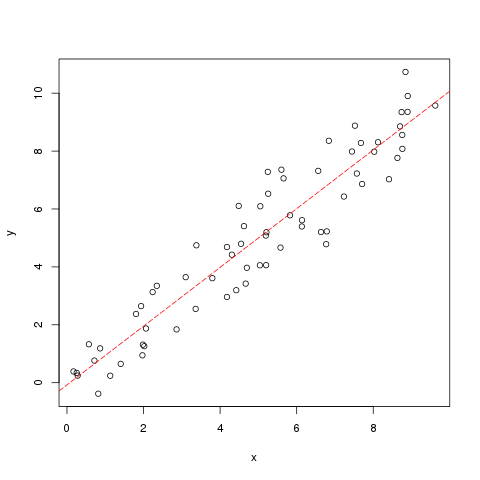
\includegraphics[scale=0.45]{a_regression/ordinary_least_squares_regression_result.png}
\caption{Plot 2D training dataset with the line of best fit.}
\label{plot:ordinary_least_squares_regression_result}
\end{figure}

% other packages ?


% References: Deeper understanding
% The references element description includes a listing of both primary sources of information about the technique as well as useful introductory sources for novices to gain a deeper understanding of the theory and application of the technique. The description consists of hand-selected reference material including books, peer reviewed conference papers, journal articles, and potentially websites. A bullet-pointed structure is suggested.
\subsection{References}
% What are the primary sources for a technique?
% What are the suggested reference sources for learning more about a technique?

% primary sources
\subsubsection{Primary Sources}
% least squares
The method for Least Squares may be traced back to Gauss who claims to have devised the method in and later published it in 1809 \cite{Gauss1809, Gauss1823} (Latin). Legendre independently developed and published the Least Squares method in 1805 \cite{Legendre1805} (Appendix, French).
% ordinary least squares specifically

% more info
\subsubsection{More Information}
% text books
Least Squares Regression is covered in any good text of statistics, data analysis or econometrics. Some popular introductory texts to least squares regression include Montgomery et~al.\ \cite{Montgomery2001} (Chapter 2), and Tamhane and Dunlop \cite{Tamhane2000} (Chapter 10).
% in R
Faraway provides a free book that includes a practical introduction into Least Squares Regression with examples in R \cite{Faraway2002} (updated version published \cite{Faraway2004}).


% END
\putbib\end{bibunit}
\newpage\begin{bibunit}% The Clever Algorithms Project: http://www.CleverAlgorithms.com
% (c) Copyright 2011 Jason Brownlee. Some Rights Reserved. 
% This work is licensed under a Creative Commons Attribution-Noncommercial-Share Alike 2.5 Australia License.

% Name
% The algorithm name defines the canonical name used to refer to the technique, in addition to common aliases, abbreviations, and acronyms. The name is used in terms of the heading and sub-headings of an algorithm description.
\section{Logistic Regression} 
\label{sec:logistic}
\index{Logistic Regression}
\index{logit}

% other names
% What is the canonical name and common aliases for a technique?
% What are the common abbreviations and acronyms for a technique?
\emph{Logistic Regression, Logit, Logit Model, Logistic Model, Binomial Logistic Regression, Binary Logistic Regression}

% Taxonomy: Lineage and locality
\subsection{Taxonomy}
% To what fields of study does a technique belong?
% What are the closely related approaches to a technique?
Logistic Regression is a regression method from the field of statistics, although us better understood as a classification method.
The most common form is Binomial Logistic Regression where the dependent variable is binary.
Logistic Regression may be considered a special case of Generalized Linear Regression.
Logistic Regression has many extensions including Ordered Logistic Regression that can handle ordinal dependent variables, and Multinomial Logistic Regression that can handle nominal (categorical) dependent variables.

What is Weighted Logistic Regression?
What is Stepwise Logistic Regression?
Where does Regularized Logistic Regression fit in?

% Strategy: Problem solving plan
% The strategy is an abstract description of the computational model. The strategy describes the information processing actions a technique shall take in order to achieve an objective. The strategy provides a logical separation between a computational realization (procedure) and a analogous system (metaphor). A given problem solving strategy may be realized as one of a number specific algorithms or problem solving systems. The strategy description is textual using information processing and algorithmic terminology.
\subsection{Strategy}
% What is the information processing objective of a technique?
Logistic Regression fits data to a logistic (sigmoidal) function and makes predictions of the probability of occurrence of an event. 
% What is a techniques plan of action?
A logistic function is used because it can take any values (positive or negative) and produce a value between 0 and 1. The logistic function is influenced by a logit function which take a variable derived from a sum of the weighted attributes. The logit function is the natural logarithm of the odds of the dependent variable equalling one.

The sign of a regression coefficient may be interpreted as the increase or decrease of an attribute to the resulting probability, and the magnitude represents the influence of the attribute.
The regression coefficients (weights) are fit by minimizing the maximum likelihood loss function. The problem as a system of linear equations use the Conjugate Gradient Method to solve the coefficients. Much research into the method is focused on more efficient algorithms for fitting the model.


% help me use this technique
\subsection{Overview}

% what it is good at
\subsubsection{Features}

\begin{itemize}
	\item Generally fast to create and results in an explainable model.
	\item Generally not parametrized, so there are no parameters to configure.
	\item Produces values always between zero and one. 
	\item Does not assume a linear relationship between the independent variables and the dependent variable. 
	\item Does not require normally distributed variables.
	\item The result is a probability of the occurrence of an event that may be interpreted as such and/or in turn be discretized to a binary classification prediction.
	\item More data can result in a better fit of the model.
	\item Training data with a minimum of 10 events per independent variable is recommended \cite{Peduzzi1996}.
	\item Features should be selected prior to fitting.
	\item Provides statistical test significance on a fitted model including: Wald Z-statistic, Likelihood-Ratio Test, and the Hosmer-Lemshow Goodness of Fit Test.
\end{itemize}

% what it is not good at
\subsubsection{Limitations}

\begin{itemize}
	\item The dependent variable must be binary (otherwise one must use another form of the method).
	\item The use of a logistic function means that input attributes can take any value, the bounds do not need to be known prior to building the model.
	\item It can only handle real-valued dependent variables.
	\item Dependent on the size of the sample used to prepare the model, smaller samples ($<1000$ or $<500$) can result in a model that overfits the training data.
	\item Solving the coefficients for large models can be very computationally expensive and remains an open area for research.
	\item Missing values must be handled explicitly or those records removed.
	\item Requires that the independent variable be related to the logit by a linear relationship.
\end{itemize}


% sample script in R
\subsection{Code Listing}
Listing~\ref{glm_logistic} provides a code listing of Logistic Regression in R using the \texttt{glm} (generalized linear model) function of the \texttt{stats} core package. 
% problem
The test problem is a contrived one dimensional problem where given a health statistic ($h$) determine whether a patient will survive or not $s\in\{0,1\}$.
The \texttt{gml} is distributed in core R and provides a number of functions besides the logistic function. By default, the method uses the Iteratively Re-weighted Least Squares (IWLS) method to fit.

% TODO make 2D problem and show the decision boundary + data points
% show stats?
% show convergence of gradient descent?

\lstinputlisting[firstline=7,language=r,caption={Example of Logistic Regression in R using the \texttt{glm} function of the \texttt{stats} core package.}, label=stats_logistic]{../src/algorithms/regression/stats_logistic_regression.R}

% References: Deeper understanding
% The references element description includes a listing of both primary sources of information about the technique as well as useful introductory sources for novices to gain a deeper understanding of the theory and application of the technique. The description consists of hand-selected reference material including books, peer reviewed conference papers, journal articles, and potentially websites. A bullet-pointed structure is suggested.
\subsection{References}
% What are the primary sources for a technique?
% What are the suggested reference sources for learning more about a technique?

% primary sources
\subsubsection{Primary Sources}

What are some primary sources for this method?

% more info
\subsubsection{More Information}
%Komarek and Moore provide promote the use of the method in modern data mining, suggesting modifications to the fit procedure to decrease computational complexity \cite{Komarek2005}.

There are many excellent books dedicated to Logistic Regression, some examples include 
``Logistic Regression: A Primer'' by Pampel that provides a practical introduction to the method \cite{Pampel2000}, ``Applied logistic regression'' by Hosmer and Lemeshow that provides a wealth of references \cite{Hosmer2000}, and ``Logistic Regression: A Self-Learning Text'' by Kleinbaum, Klein, and Pryor that is also an excellent self-paced introductory text \cite{Kleinbaum2010}.


% END\putbib\end{bibunit}
\newpage\begin{bibunit}% The Clever Algorithms Project: http://www.CleverAlgorithms.com
% (c) Copyright 2013 Jason Brownlee. Some Rights Reserved. 
% This work is licensed under a Creative Commons Attribution-Noncommercial-Share Alike 2.5 Australia License.


% Name
% The algorithm name defines the canonical name used to refer to the technique, in addition to common aliases, abbreviations, and acronyms. The name is used in terms of the heading and sub-headings of an algorithm description.
\section{Ridge Regression} 
\label{sec:ridge}
\index{Ridge Regression}
\index{Tikhonov Regularization}
\index{Tikhonov-Miller Method}
\index{Phillips-Twomey Method}
\index{Constrained Linear Inversion}
\index{Linear Regularization}
\index{Penalized $L_2$ Regression}
\index{$L_2$-norm Penalty}

% other names
% What is the canonical name and common aliases for a technique?
% What are the common abbreviations and acronyms for a technique?
\emph{Ridge Regression, Tikhonov Regularization, Tikhonov-Miller Method, Phillips-Twomey Method, Constrained Linear Inversion, Linear Regularization, Penalized $L_2$ Regression}

% Taxonomy: Lineage and locality
% The algorithm taxonomy defines where a techniques fits into the field, both the specific subfields of Computational Intelligence and Biologically Inspired Computation as well as the broader field of Artificial Intelligence. The taxonomy also provides a context for determining the relation- ships between algorithms. The taxonomy may be described in terms of a series of relationship statements or pictorially as a venn diagram or a graph with hierarchical structure.
\subsection{Taxonomy}
% To what fields of study does a technique belong?
Ridge Regression is a Regularization method for Multiple Linear Regression models.
% What are the closely related approaches to a technique?
Ridge Regression is related to other Regularized Regression models such as the LASSO and Elastic Net.
The general method of penalizing a model based on the sum of squared parameters is related to Weight Decay in the training of Artificial Neural Networks.

% Strategy: Problem solving plan
% The strategy is an abstract description of the computational model. The strategy describes the information processing actions a technique shall take in order to achieve an objective. The strategy provides a logical separation between a computational realization (procedure) and a analogous system (metaphor). A given problem solving strategy may be realized as one of a number specific algorithms or problem solving systems. The strategy description is textual using information processing and algorithmic terminology.
\subsection{Strategy}
% What is the information processing objective of a technique?
The information processing objective of Ridge Regression is to reduce or shrink the magnitude of the coefficients in a regression model.
% What is a techniques plan of action?
This is achieved by penalizing models based on the sum of the squared coefficients called an $L_2$ penalty or the $L_2$ norm. This term is added to the regression equation during the preparation of the model and is weighted by a complexity parameter ($\lambda$) that controls the amount of shrinkage of the coefficients. 
The effect is that coefficients of a regression model are shrunk towards zero during the training of the model. The intercept is not penalized.

% Heuristics: Usage guidelines
% The heuristics element describe the commonsense, best practice, and demonstrated rules for applying and configuring a parameterized algorithm. The heuristics relate to the technical details of the techniques procedure and data structures for general classes of application (neither specific implementations not specific problem instances). The heuristics are described textually, such as a series of guidelines in a bullet-point structure.
\subsection{Heuristics}
% What are the suggested configurations for a technique?
% What are the guidelines for the application of a technique to a problem instance?

\begin{itemize}
	\item It commonly results in a model with a better bias-variance trade-off than Ordinary Least Squares.
	\item The ridge constant $\lambda$ is typically selected in the range $[0,1]$, where $\lambda=0$ corresponds to an Ordinary Least Squares regression.
	\item Unlike other selection methods, Ridge Regression does not drop coefficients, all model parameters are maintained at the end of the process providing shrinkage but not selection of parameters.
	\item Inputs are commonly standardized before training the model as models are not equivalent under scaling.
	\item Cross-validation is commonly used to assess the model and model selection or stopping criteria.
	\item It is suited for problems where there are more predictors $p$ than there are observations $n$, $p>n$ problems.
\end{itemize}

% sample script in R
\subsection{Code Listing}
% listing
Listing~\ref{mass_ridge_regression} provides a code listing of the Ridge Regression method in R.
% algorithm and package
The example uses the \texttt{lm.ridge()} function in the \texttt{MASS} core package which is responsible for fitting linear models using Ridge Regression. The example trials a sequence of lambda values then uses the model with the best lambda value for prediction. Figure~\ref{plot:ridge_regression_result} provides a plot of the final coefficient values of each model for the given lambda values. For more information on this library type: \texttt{library(help="MASS")}, and for more information on the function type: \texttt{?lm.ridge}.

% problem
The test problem is a four-dimensional dataset of 100 samples, where \texttt{x3} and \texttt{y} are dependent on \texttt{x1} and \texttt{x1} and \texttt{x2} are independent variables. The problem is ill defined as \texttt{y} given \texttt{x1, x2, x3}. The model is expected to reduce the contribution of \texttt{x2} and \texttt{x3} toward zero leaving \texttt{y} given \texttt{x1}.

\lstinputlisting[firstline=7,language=r,caption={Example of Ridge Regression in R using the \texttt{lm.ridge()} function in the \texttt{MASS} package.}, label=mass_ridge_regression]{../src/algorithms/regularization/mass_ridge_regression.R}

\begin{figure}[htp]
\centering
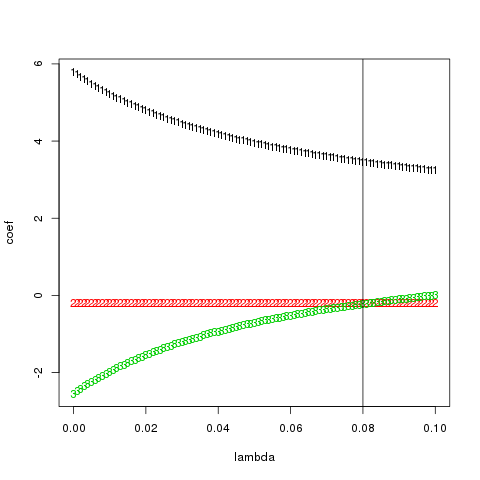
\includegraphics[scale=0.70]{book/a_regularization/ridge_regression_result.png}
\caption{Plot of the final coefficient values of each model for the given lambda values. The numbers reflect the \texttt{x} variables 1, 2 and 3. The line shows a selected lambda value.}
\label{plot:ridge_regression_result}
\end{figure}

% other packages ?
Other packages that provide an implementation of Ridge Regression include \texttt{parcor}.
% penalized package

% References: Deeper understanding
% The references element description includes a listing of both primary sources of information about the technique as well as useful introductory sources for novices to gain a deeper understanding of the theory and application of the technique. The description consists of hand-selected reference material including books, peer reviewed conference papers, journal articles, and potentially websites. A bullet-pointed structure is suggested.
\subsection{References}
% What are the primary sources for a technique?
% What are the suggested reference sources for learning more about a technique?

% primary sources
\subsubsection{Primary Sources}
% seminal
The method was originally described by Tikhonov \cite{Tikhonov1943, Tikhonov1963} (Russian), who later published a full account of the method as a book \cite{Tikhonov1977}.
% others
Phillips independently described the method \cite{Phillips1962}. Hoerl was first to use the term `Ridge Regression' which was adopted in the field of Statistics for $p>n$ problems \cite{Hoerl1962, Hoerl1970, Hoerl1970a}.

% more info
\subsubsection{More Information}
Hastie et~al.\ provide a gentle introduction to the method from the perspective of linear regression (\cite{Hastie2009}, page 61).
% applied
Press et~al.\ provide an introduction to Ridge Regression with examples in the C programming language \cite{Press2007} (Chapter 19).
Faraway provides an introduction to Ridge Regression with examples in R \cite{Faraway2002}.

% END
\putbib\end{bibunit}
\newpage\begin{bibunit}% The Clever Algorithms Project: http://www.CleverAlgorithms.com
% (c) Copyright 2011 Jason Brownlee. Some Rights Reserved. 
% This work is licensed under a Creative Commons Attribution-Noncommercial-Share Alike 2.5 Australia License.

% Name
% The algorithm name defines the canonical name used to refer to the technique, in addition to common aliases, abbreviations, and acronyms. The name is used in terms of the heading and sub-headings of an algorithm description.
\section{Stepwise Linear Regression} 
\label{sec:stepwise}
\index{Stepwise Linear Regression}

% other names
% What is the canonical name and common aliases for a technique?
% What are the common abbreviations and acronyms for a technique?
\emph{Stepwise Linear Regression, Stepwise Selection}

% Taxonomy: Lineage and locality
% The algorithm taxonomy defines where a techniques fits into the field, both the specific subfields of Computational Intelligence and Biologically Inspired Computation as well as the broader field of Artificial Intelligence. The taxonomy also provides a context for determining the relation- ships between algorithms. The taxonomy may be described in terms of a series of relationship statements or pictorially as a venn diagram or a graph with hierarchical structure.
\subsection{Taxonomy}
% To what fields of study does a technique belong?
% What are the closely related approaches to a technique?
Stepwise Regression is a model selection method for selecting a regression model. It is typically applied to Linear Regression and Generalized Linear Regression Models.

% Strategy: Problem solving plan
% The strategy is an abstract description of the computational model. The strategy describes the information processing actions a technique shall take in order to achieve an objective. The strategy provides a logical separation between a computational realization (procedure) and a analogous system (metaphor). A given problem solving strategy may be realized as one of a number specific algorithms or problem solving systems. The strategy description is textual using information processing and algorithmic terminology.
\subsection{Strategy}
% What is the information processing objective of a technique?
% What is a techniques plan of action?

used for feature selection
greedy algorithm - adds the best feature or removes the worst feature each iteration
have to decide when to stop the algorithm - stopping condition - typically done by cross validation
some criteria can be optimized

see \url{http://www.stata.com/support/faqs/stat/stepwise.html}
good example \url{http://cran.r-project.org/doc/contrib/Faraway-PRA.pdf}

% help me use this technique
\subsection{Overview}

% what it is good at
\subsubsection{Features}

\begin{itemize}
	\item Simple method for feature selection.
	\item One of a variety of selection criteria can be used, common examples include the Akaike Information Criterion (AIC), and the Bayes Information Criterion (BIC).
\end{itemize}

% what it is not good at
\subsubsection{Limitations}

\begin{itemize}
	\item Stepwise models are a deprecated method as they have a high chance of selecting the wrong attributes and being optimistic of the model they prepare.
\end{itemize}



% sample script in R
\subsection{Code Listing}
% listing
Listing~\ref{stats_stepwise_linear_regression} provides a code listing of Stepwise Linear Regression method in R to find the relevant features and the line of best fit for those features.
% algorithm and package
The example uses the {lm()} function and the and \texttt{step()} in the \texttt{stats} core package which are responsible for fitting linear models and performing stepwise selection respectively. The \texttt{step()} function uses a Akaike Information Criterion as the model evaluation criteria.

% problem
The test problem is a four-dimensional dataset of 50 samples, where the x-values are drawn from a uniformly random distribution $x \in [0,10]$ and \texttt{y} values are dependent on the \texttt{x} value plus a value drawn from a normally random distribution with a mean of 0 and a standard deviation of 1. The features \texttt{a} and \texttt{b} are random independent variables that have no relevant interaction x and y. In this example, \texttt{y} is considered the dependent variable and x the single relevant independent. The stepwise method is expected to discount \texttt{a} and \texttt{b} and select a linear model for \texttt{y} given \texttt{x}.

% classification example?

\lstinputlisting[firstline=7,language=r,caption={Example of Stepwise Linear Regression in R using the \texttt{lm()} and \texttt{step()} functions in the \texttt{stats} core package.}, label=stats_stepwise_linear_regression]{../src/algorithms/regression/stats_stepwise_linear_regression.R}

% other packages
Other packages that provide stepwise selection include the \texttt{stepAIC} function of the \texttt{MASS} package. The \texttt{leaps} package does not provide stepwise selection, although does provides a related selection method called Regression Subset Selection that uses a branch and bound search.


% References: Deeper understanding
% The references element description includes a listing of both primary sources of information about the technique as well as useful introductory sources for novices to gain a deeper understanding of the theory and application of the technique. The description consists of hand-selected reference material including books, peer reviewed conference papers, journal articles, and potentially websites. A bullet-pointed structure is suggested.
\subsection{References}
% What are the primary sources for a technique?
% What are the suggested reference sources for learning more about a technique?

% primary sources
\subsubsection{Primary Sources}


Great early overview of the approaches (forward and backward selection) \cite{Hocking1976}.

% more info
\subsubsection{More Information}

arguments against it in modern analysis
Overview of why using stepwise regression is a bad idea \cite{Whittingham2006}.
\cite{Mundry2009}





% END
\putbib\end{bibunit}
\newpage\begin{bibunit}% The Clever Algorithms Project: http://www.CleverAlgorithms.com
% (c) Copyright 2011 Jason Brownlee. Some Rights Reserved. 
% This work is licensed under a Creative Commons Attribution-Noncommercial-Share Alike 2.5 Australia License.

% Name
% The algorithm name defines the canonical name used to refer to the technique, in addition to common aliases, abbreviations, and acronyms. The name is used in terms of the heading and sub-headings of an algorithm description.
\section{Multivariate Adaptive Regression Splines} 
\label{sec:mars}
\index{Multivariate Adaptive Regression Splines}
\index{MARS}

% other names
% What is the canonical name and common aliases for a technique?
% What are the common abbreviations and acronyms for a technique?
\emph{Multivariate Adaptive Regression Splines, MARS.}

% Taxonomy: Lineage and locality
% The algorithm taxonomy defines where a techniques fits into the field, both the specific subfields of Computational Intelligence and Biologically Inspired Computation as well as the broader field of Artificial Intelligence. The taxonomy also provides a context for determining the relation- ships between algorithms. The taxonomy may be described in terms of a series of relationship statements or pictorially as a venn diagram or a graph with hierarchical structure.
\subsection{Taxonomy}
% To what fields of study does a technique belong?
% What are the closely related approaches to a technique?
Multivariate Adaptive Regression Splines is a regression method.


% Strategy: Problem solving plan
% The strategy is an abstract description of the computational model. The strategy describes the information processing actions a technique shall take in order to achieve an objective. The strategy provides a logical separation between a computational realization (procedure) and a analogous system (metaphor). A given problem solving strategy may be realized as one of a number specific algorithms or problem solving systems. The strategy description is textual using information processing and algorithmic terminology.
\subsection{Strategy}
% What is the information processing objective of a technique?
% What is a techniques plan of action?

generalization of stepwise linear regression?


% Heuristics: Usage guidelines
% The heuristics element describe the commonsense, best practice, and demonstrated rules for applying and configuring a parameterized algorithm. The heuristics relate to the technical details of the techniques procedure and data structures for general classes of application (neither specific implementations not specific problem instances). The heuristics are described textually, such as a series of guidelines in a bullet-point structure.
\subsection{Heuristics}
% What are the suggested configurations for a technique?
% What are the guidelines for the application of a technique to a problem instance?

\begin{itemize}
	\item 
\end{itemize}

% sample script in R
\subsection{Code Listing}

MASS package
earth package
mda package

% References: Deeper understanding
% The references element description includes a listing of both primary sources of information about the technique as well as useful introductory sources for novices to gain a deeper understanding of the theory and application of the technique. The description consists of hand-selected reference material including books, peer reviewed conference papers, journal articles, and potentially websites. A bullet-pointed structure is suggested.
\subsection{References}
% What are the primary sources for a technique?
% What are the suggested reference sources for learning more about a technique?

% primary sources
\subsubsection{Primary Sources}



% more info
\subsubsection{More Information}





% END
\putbib\end{bibunit}
\newpage\begin{bibunit}% The Clever Algorithms Project: http://www.CleverAlgorithms.com
% (c) Copyright 2011 Jason Brownlee. Some Rights Reserved. 
% This work is licensed under a Creative Commons Attribution-Noncommercial-Share Alike 2.5 Australia License.

% Name
% The algorithm name defines the canonical name used to refer to the technique, in addition to common aliases, abbreviations, and acronyms. The name is used in terms of the heading and sub-headings of an algorithm description.
\section{Linear Discriminant Analysis} 
\label{sec:lda}
\index{Linear Discriminant Analysis}
\index{Discriminant Analysis}
\index{LDA}

% other names
% What is the canonical name and common aliases for a technique?
% What are the common abbreviations and acronyms for a technique?
\emph{Linear Discriminant Analysis, Discriminant Analysis, Discriminant Function Analysis, LDA.}

% Taxonomy: Lineage and locality
% The algorithm taxonomy defines where a techniques fits into the field, both the specific subfields of Computational Intelligence and Biologically Inspired Computation as well as the broader field of Artificial Intelligence. The taxonomy also provides a context for determining the relation- ships between algorithms. The taxonomy may be described in terms of a series of relationship statements or pictorially as a venn diagram or a graph with hierarchical structure.
\subsection{Taxonomy}
% To what fields of study does a technique belong?
% What are the closely related approaches to a technique?
Linear Discriminant Analysis is a XXX method.

% Strategy: Problem solving plan
% The strategy is an abstract description of the computational model. The strategy describes the information processing actions a technique shall take in order to achieve an objective. The strategy provides a logical separation between a computational realization (procedure) and a analogous system (metaphor). A given problem solving strategy may be realized as one of a number specific algorithms or problem solving systems. The strategy description is textual using information processing and algorithmic terminology.
\subsection{Strategy}
% What is the information processing objective of a technique?
% What is a techniques plan of action?

used for classification and dimensionality redunction
kind of like regression


% Heuristics: Usage guidelines
% The heuristics element describe the commonsense, best practice, and demonstrated rules for applying and configuring a parameterized algorithm. The heuristics relate to the technical details of the techniques procedure and data structures for general classes of application (neither specific implementations not specific problem instances). The heuristics are described textually, such as a series of guidelines in a bullet-point structure.
\subsection{Heuristics}
% What are the suggested configurations for a technique?
% What are the guidelines for the application of a technique to a problem instance?

\begin{itemize}
	\item 
\end{itemize}


% References: Deeper understanding
% The references element description includes a listing of both primary sources of information about the technique as well as useful introductory sources for novices to gain a deeper understanding of the theory and application of the technique. The description consists of hand-selected reference material including books, peer reviewed conference papers, journal articles, and potentially websites. A bullet-pointed structure is suggested.
\subsection{References}
% What are the primary sources for a technique?
% What are the suggested reference sources for learning more about a technique?

% primary sources
\subsubsection{Primary Sources}



% more info
\subsubsection{More Information}





% END
\putbib\end{bibunit}


